\section{Pruebas de la aplicación}

    \subsection{Pruebas de Rendimiento}

        \subsubsection{Dispositivos de prueba}

            Con el fin de evaluar el funcionamiento del aplicativo en diferentes condiciones de hardware, las pruebas se realizaron en tres dispositivos Android correspondientes a las gamas baja, media y alta. En todos los casos, la tasa de refresco de la pantalla se configuró a 60 Hz para mantener las mismas condiciones durante la ejecución de las pruebas.

            La Tabla \ref{tab:devices_specs} presenta las principales especificaciones técnicas de los dispositivos utilizados para la evaluación del aplicativo.

            \begin{ThreePartTable}

    \renewcommand\TPTminimum{\textwidth}

    \setlength\LTleft{0pt}
    \setlength\LTright{0pt}
    \setlength\tabcolsep{3pt}

    \begin{TableNotes}
        \item \textbf{Nota.} Especificaciones técnicas obtenidas de los metadatos de ejecución generados por la herramienta Macrobenchmark de Jetpack y de las fichas técnicas oficiales de cada fabricante.
    \end{TableNotes}

    \begin{longtable}{@{}P{0.15\textwidth}P{0.20\textwidth}P{0.22\textwidth}P{0.15\textwidth}P{0.10\textwidth}P{0.10\textwidth}@{}}

        \caption{Especificaciones técnicas de los dispositivos de prueba} \label{tab:devices_specs} \\

        \toprule
        \textbf{Marca} &
            \textbf{Modelo} &
                \textbf{SoC} &
                    \textbf{Núcleos} &
                        \textbf{RAM} &
                            \textbf{Android} \\
        \toprule
        \endfirsthead

        \multicolumn{6}{r}{\textit{(Continuación de la Tabla \ref{tab:devices_specs})}} \\
        \toprule
        \textbf{Marca} &
            \textbf{Modelo} &
                \textbf{SoC} &
                    \textbf{Núcleos} &
                        \textbf{RAM} &
                            \textbf{Android} \\
        \toprule
        \endhead

        \midrule[\heavyrulewidth]
        \multicolumn{6}{r}{\textit{Continúa en la siguiente página}}\\
        \endfoot

        \bottomrule
        \insertTableNotes\\
        \endlastfoot

        Motorola &
            Moto G15 &
                Mediatek Helio G81 Extreme (12 nm) &
                    Octa-core 2.0 GHz &
                        4 GB &
                            15 \\

        \midrule

        Xiaomi &
            Redmi Note 10 Pro &
                Snapdragon 732G (8 nm) &
                    Octa-core 2.3 GHz &
                        8 GB &
                            13 \\

        \midrule

        OPPO &
            Reno14 F &
                Snapdragon 6 Gen 1 (4 nm) &
                    Octa-core 2.2 GHz &
                        12 GB &
                            15 \\

    \end{longtable}

\end{ThreePartTable}

        \subsubsection{Pruebas de tiempo de inicio (Startup)}

            El tiempo de inicio de una aplicación constituye uno de los principales indicadores de la experiencia de uso, ya que corresponde al tiempo que transcurre desde que el usuario solicita la apertura del aplicativo hasta que este se encuentra disponible para su utilización. Para evaluar este comportamiento, se realizaron pruebas en tres escenarios de arranque que representan diferentes estados del aplicativo dentro del sistema operativo Android.

            Para cada uno de estos tres escenarios, se ejecutaron diez iteraciones por dispositivo utilizando la herramienta \textit{Macrobenchmark} de Jetpack, registrando el tiempo total de inicio en milisegundos (ms) mediante la métrica \textit{StartupTimingMetric}. A partir de las mediciones obtenidas se calcularon los valores de tiempo mínimo, máximo y promedio, mediante un gráfico de barras que contrasta el rendimiento de inicio entre los tres dispositivos evaluados.

            \paragraph{Cold Start (Arranque en frío)}

                Este escenario ocurre cuando el proceso de la aplicación no se encuentra en memoria y el sistema operativo debe inicializarlo completamente. En consecuencia, representa el caso de mayor tiempo de inicio, ya que requiere crear el proceso, cargar los recursos principales e iniciar la actividad inicial del aplicativo. Los resultados obtenidos para este escenario se presentan en la Figura \ref{fig:benchmark_startup_cold}.

                \begin{figure}[H]
    \caption{Comparación de tiempos de inicio en frío}
    \centering
    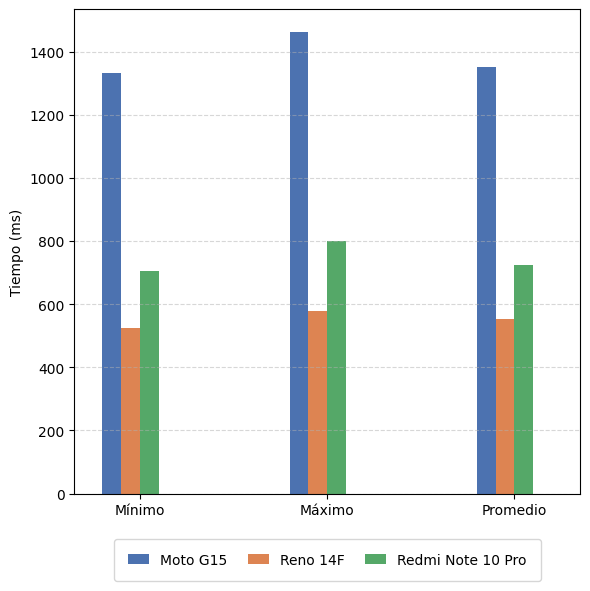
\includegraphics[width=0.8\textwidth]{assets/figures/third_phase/benchmark/img_benchmark_startup_cold.png}
    \label{fig:benchmark_startup_cold}
\end{figure}
\fixvspace{0}

            \paragraph{Warm Start (Arranque templado)}

                Corresponde al escenario en el que el proceso del aplicativo permanece activo en memoria, pero la actividad principal debe reconstruirse antes de mostrarse nuevamente al usuario. Debido a que el proceso ya existe, el tiempo de inicio es menor que en un arranque en frío. La comparación entre los dispositivos evaluados para este tipo de arranque se presenta en la Figura \ref{fig:benchmark_startup_warm}.

                \begin{figure}[H]
    \caption{Comparación de tiempo de inicio en templado (Warm Startup) por dispositivo}
    \centering
    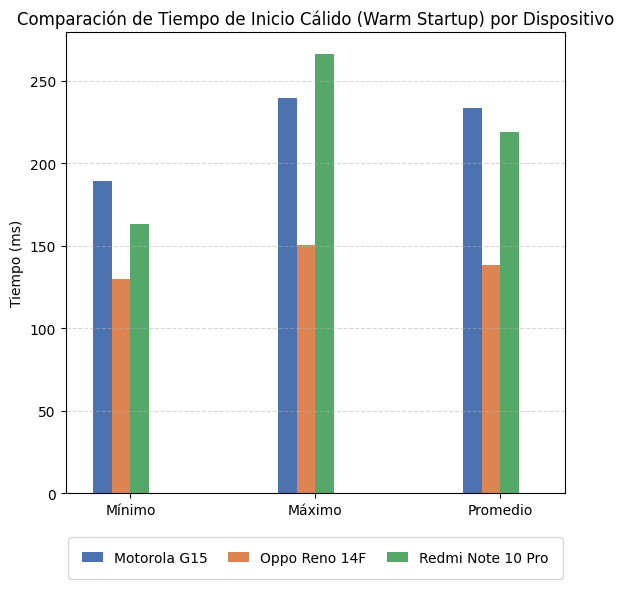
\includegraphics[width=0.6\textwidth]{assets/figures/third_phase/benchmark/img_benchmark_startup_warm.png}
    \label{fig:benchmark_startup_warm}
\end{figure}
\fixvspace{0}

            \paragraph{Hot Start (Arranque en caliente)}

                En este caso, tanto el proceso como la actividad permanecen residentes en memoria, por lo que el sistema únicamente devuelve la aplicación al primer plano. Este escenario representa el menor tiempo de inicio y corresponde a situaciones en las que el usuario cambia temporalmente de aplicación y regresa inmediatamente al aplicativo. Los resultados de esta prueba se muestran en la Figura \ref{fig:benchmark_startup_hot}.

                \begin{figure}[H]
    \caption{Comparación de tiempo de inicio en caliente (Hot Startup) por dispositivo}
    \centering
    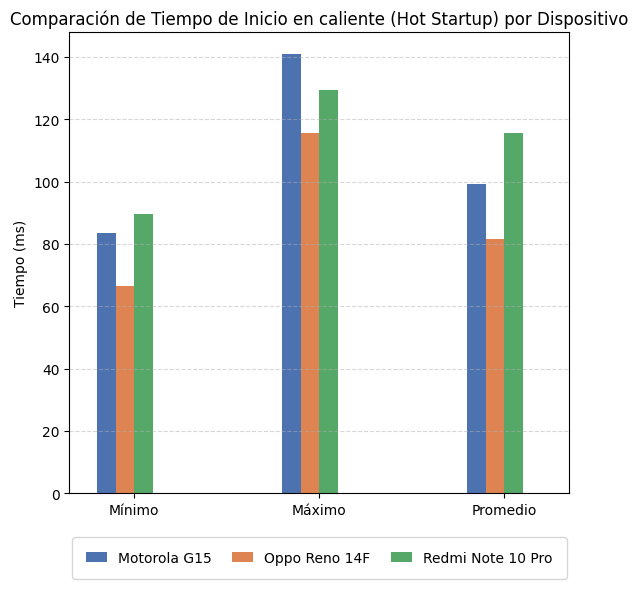
\includegraphics[width=0.6\textwidth]{assets/figures/third_phase/benchmark/img_benchmark_startup_hot.png}
    \label{fig:benchmark_startup_hot}
\end{figure}
\fixvspace{0}

        \subsubsection{Pruebas de navegación entre pantallas}

            Con el propósito de evaluar el comportamiento del aplicativo durante la navegación, se analizaron tres recorridos distintos desde la pantalla principal hasta las interfaces relacionadas con la configuración y ejecución de las actividades de realidad aumentada. Estas pruebas permiten comparar el desempeño del aplicativo en dispositivos con diferentes capacidades de hardware durante la carga y transición entre pantallas.

            Para este análisis se emplearon dos métricas proporcionadas por la herramienta \textit{Macrobenchmark}: la duración de cuadro (\textit{Frame Duration}) y el sobrepaso de cuadro (\textit{Frame Overrun}).

            \begin{itemize}
                \item \textbf{Frame Duration (\textit{frameDurationCpuMs}):} corresponde al tiempo, medido en milisegundos, que requiere la CPU para procesar y renderizar cada cuadro durante la navegación entre pantallas.

                \item \textbf{Frame Overrun (\textit{frameOverrunMs}):} representa la diferencia entre el tiempo requerido para procesar un cuadro y el tiempo disponible para mantener una frecuencia de actualización de 60 Hz. Valores positivos indican que el tiempo disponible fue excedido, mientras que valores negativos o iguales a cero indican que el procesamiento se realizó dentro del margen esperado.
            \end{itemize}

            Los resultados se presentan mediante los percentiles P50, P90, P95 y P99, permitiendo comparar tanto el comportamiento habitual de la navegación como aquellos casos en los que se presentan los mayores tiempos de procesamiento.

            \paragraph{Navegación hacia la sesión de realidad aumentada}

                La primera prueba corresponde al recorrido desde la pantalla principal hasta la sesión de realidad aumentada. Los resultados obtenidos para los tres dispositivos se presentan en la Figura \ref{fig:benchmark_nav_to_arsession}.

                \begin{figure}[H]
    \caption{Duración del fotograma en la transición y apertura de la sesión de RA por percentil y dispositivo}
    \centering
    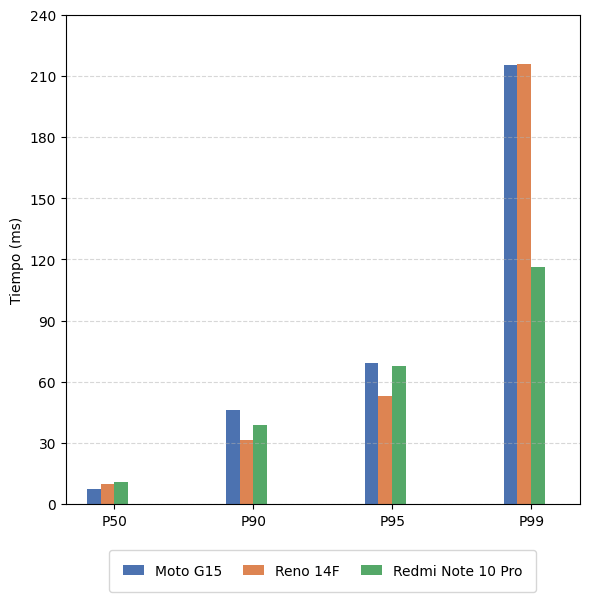
\includegraphics[width=0.6\textwidth]{assets/figures/third_phase/benchmark/img_benchmark_navigation_to_arsession.png}
    \label{fig:benchmark_nav_to_arsession}
\end{figure}
\fixvspace{0}

            \paragraph{Navegación hacia la pantalla de calibración}

                La segunda prueba evalúa la navegación desde la pantalla principal hasta la interfaz de calibración de modelos 3D. La comparación entre los dispositivos evaluados se presenta en la Figura \ref{fig:benchmark_nav_to_calibration}.

                \begin{figure}[H]
    \caption{Duración del fotograma en la transición y apertura de la calibración de RA por percentil y dispositivo}
    \centering
    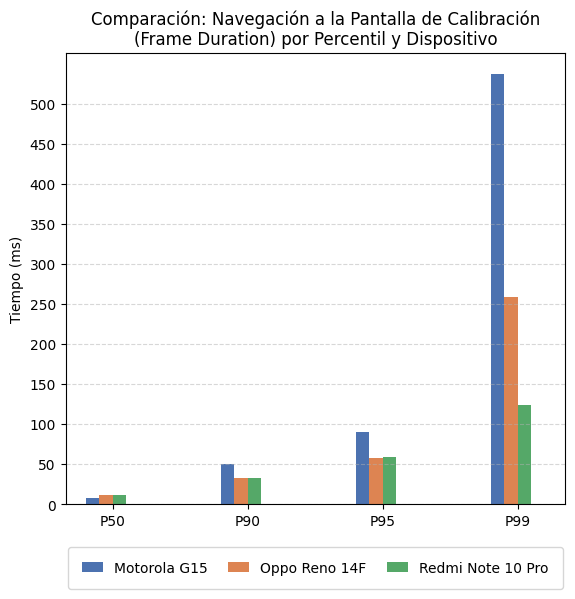
\includegraphics[width=0.6\textwidth]{assets/figures/third_phase/benchmark/img_benchmark_navigation_to_calibration.png}
    \label{fig:benchmark_nav_to_calibration}
\end{figure}
\fixvspace{0}

            \paragraph{Navegación hacia el editor de actividades}

                La última prueba analiza el recorrido desde la pantalla principal hasta el editor de actividades de mantenimiento, donde se configuran los pasos y operaciones asociados a cada procedimiento. Los resultados obtenidos se muestran en la Figura \ref{fig:benchmark_nav_to_editor}.

                \begin{figure}[H]
    \caption{Comparación de navegación a la pantalla de editor de actividades}
    \centering
    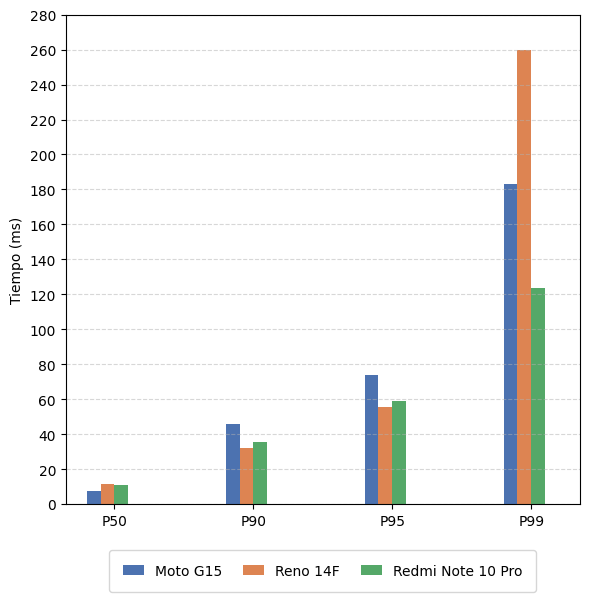
\includegraphics[width=0.6\textwidth]{assets/figures/third_phase/benchmark/img_benchmark_navigation_to_editor.png}
    \label{fig:benchmark_nav_to_editor}
\end{figure}
\fixvspace{0}

    \subsection{Pruebas de funcionamiento de las pantallas}

        \subsubsection{Funcionamiento de las pantallas de información técnica}

            \paragraph{Pantalla de especificaciones}
            \paragraph{Pantalla de documentación}
            \paragraph{Pantalla de actividades de mantenimiento}

        \subsubsection{Funcionamiento de las pantallas de configuración previa de realidad aumentada}

            \paragraph{Pantalla de marcadores}
            \paragraph{Pantalla de calibración de modelos 3D}
            \paragraph{Pantalla de editor de actividades de mantenimiento}

        \subsubsection{Funcionamiento de la pantalla final de sesión de realidad aumentada}